% =============================================================================
% cover-schieberegister.tex – Standalone Cover für techdoc.cls
% =============================================================================
% Kompilieren: xelatex cover-schieberegister.tex
% Erzeugt: cover-schieberegister.pdf (für \coverimage in main.tex)
% Inhalt: CD4021B + 74HC595 Bit-Mapping (kompakt)
% =============================================================================
\documentclass[tikz,border=0pt]{standalone}

% -----------------------------------------------------------------------------
% SCHRIFTEN (identisch mit techdoc.cls)
% -----------------------------------------------------------------------------
\usepackage{fontspec}
\defaultfontfeatures{Ligatures=TeX}

% TeX Gyre Schriften (Standard in TeX Live)
\setmainfont{TeX Gyre Pagella}
\setsansfont{TeX Gyre Heros}
\setmonofont[Scale=0.85]{TeX Gyre Cursor}

% -----------------------------------------------------------------------------
% FARBEN (identisch mit techdoc.cls)
% -----------------------------------------------------------------------------
\usepackage{xcolor}
\definecolor{ArduinoTeal}{HTML}{00979D}
\definecolor{ArduinoDark}{HTML}{005C5F}
\definecolor{RaspberryRed}{HTML}{C51A4A}
\definecolor{SuccessGreen}{HTML}{75A928}
\definecolor{WarningOrange}{HTML}{D97706}
\definecolor{MutedText}{HTML}{4A5568}
\definecolor{CodeBg}{HTML}{F8FAFC}
\definecolor{CodeFrame}{HTML}{C8D2DC}

% -----------------------------------------------------------------------------
% TIKZ-BIBLIOTHEKEN
% -----------------------------------------------------------------------------
\usetikzlibrary{shapes, arrows.meta, positioning, calc, decorations.pathreplacing}

\begin{document}
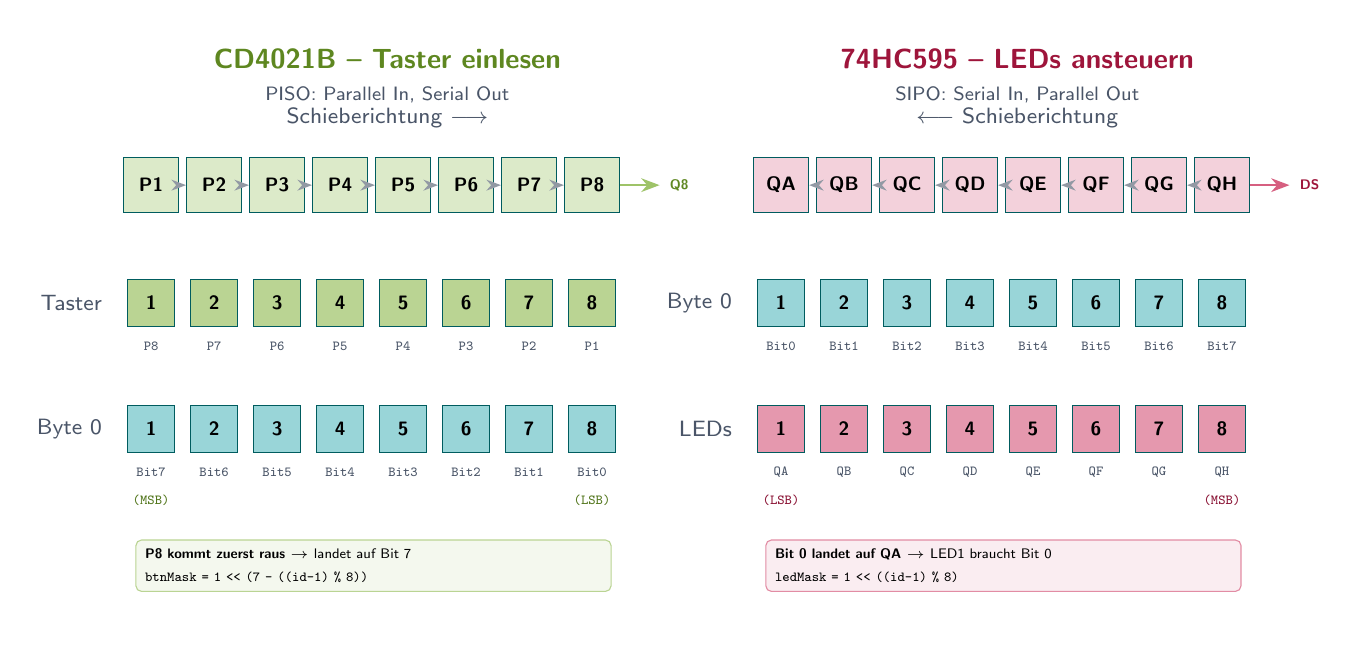
\begin{tikzpicture}[
  % Grundstile
  flipflop/.style={
    draw=ArduinoDark,
    fill=#1,
    minimum width=0.7cm,
    minimum height=0.7cm,
    font=\sffamily\bfseries\scriptsize
  },
  flipflop/.default=white,
  bitbox/.style={
    draw=ArduinoDark,
    fill=#1,
    minimum width=0.6cm,
    minimum height=0.6cm,
    font=\sffamily\bfseries\scriptsize
  },
  bitbox/.default=ArduinoTeal!30,
  lbl/.style={
    font=\sffamily\footnotesize,
    color=MutedText
  },
  bitlbl/.style={
    font=\ttfamily\tiny,
    color=MutedText
  },
  chainarrow/.style={
    draw=MutedText!60,
    line width=0.5pt,
    ->,
    >=Stealth
  }
]

% =============================================================================
% HINTERGRUND
% =============================================================================
\fill[white] (-1,-0.8) rectangle (15,7);

% =============================================================================
% LINKE SEITE: CD4021B – PISO (Parallel In, Serial Out)
% =============================================================================
\node[font=\sffamily\bfseries, color=SuccessGreen!80!black] at (3.2,6.6) {CD4021B – Taster einlesen};
\node[font=\sffamily\scriptsize, color=MutedText] at (3.2,6.15) {PISO: Parallel In, Serial Out};
\node[lbl, anchor=south] at (3.2,5.6) {Schieberichtung $\longrightarrow$};

% Schiebekette CD4021
\foreach \i/\pin in {0/P1, 1/P2, 2/P3, 3/P4, 4/P5, 5/P6, 6/P7, 7/P8} {
  \node[flipflop=SuccessGreen!25] (ff\i) at (\i*0.8+0.2,5) {\pin};
}
% Pfeile zwischen Flip-Flops
\foreach \i in {0,...,6} {
  \pgfmathtruncatemacro{\j}{\i+1}
  \draw[chainarrow] (ff\i.east) -- (ff\j.west);
}
% Ausgang Q8
\draw[chainarrow, line width=0.8pt, draw=SuccessGreen!70] (ff7.east) -- ++(0.5,0) node[right, font=\sffamily\tiny\bfseries, color=SuccessGreen!80!black] {Q8};

% Verdrahtung: Taster → Pins
\node[lbl, anchor=east] at (-0.3,3.5) {Taster};
\foreach \i/\btn in {0/1, 1/2, 2/3, 3/4, 4/5, 5/6, 6/7, 7/8} {
  \node[bitbox=SuccessGreen!50] (btn\i) at (\i*0.8+0.2,3.5) {\btn};
}
\foreach \i/\pin in {0/P8, 1/P7, 2/P6, 3/P5, 4/P4, 5/P3, 6/P2, 7/P1} {
  \node[bitlbl] at (\i*0.8+0.2,2.95) {\pin};
}

% Ergebnis: Empfangenes Byte
\node[lbl, anchor=east] at (-0.3,1.9) {Byte 0};
\foreach \i/\btn in {0/1, 1/2, 2/3, 3/4, 4/5, 5/6, 6/7, 7/8} {
  \node[bitbox=ArduinoTeal!40] (out\i) at (\i*0.8+0.2,1.9) {\btn};
}
\foreach \i/\bit in {0/Bit7, 1/Bit6, 2/Bit5, 3/Bit4, 4/Bit3, 5/Bit2, 6/Bit1, 7/Bit0} {
  \node[bitlbl] at (\i*0.8+0.2,1.35) {\bit};
}
\node[bitlbl, color=SuccessGreen!70!black] at (0.2,1.0) {(MSB)};
\node[bitlbl, color=SuccessGreen!70!black] at (5.8,1.0) {(LSB)};

% Hinweis-Box CD4021
\node[draw=SuccessGreen!50, fill=SuccessGreen!8, rounded corners=2pt,
      font=\sffamily\tiny, text width=5.8cm, align=left,
      anchor=north west] at (0,0.5) {
  \textbf{P8 kommt zuerst raus} $\rightarrow$ landet auf Bit 7\\[2pt]
  \texttt{btnMask = 1 << (7 - ((id-1) \% 8))}
};

% =============================================================================
% RECHTE SEITE: 74HC595 – SIPO (Serial In, Parallel Out)
% =============================================================================
\node[font=\sffamily\bfseries, color=RaspberryRed!80!black] at (11.2,6.6) {74HC595 – LEDs ansteuern};
\node[font=\sffamily\scriptsize, color=MutedText] at (11.2,6.15) {SIPO: Serial In, Parallel Out};
\node[lbl, anchor=south] at (11.2,5.6) {$\longleftarrow$ Schieberichtung};

% Schiebekette 74HC595
\foreach \i/\out in {0/QA, 1/QB, 2/QC, 3/QD, 4/QE, 5/QF, 6/QG, 7/QH} {
  \node[flipflop=RaspberryRed!20] (sr\i) at (\i*0.8+8.2,5) {\out};
}
% Pfeile zwischen Flip-Flops (rückwärts)
\foreach \i in {1,...,7} {
  \pgfmathtruncatemacro{\j}{\i-1}
  \draw[chainarrow] (sr\i.west) -- (sr\j.east);
}
% Eingang DS
\draw[chainarrow, line width=0.8pt, draw=RaspberryRed!70] (sr7.east) -- ++(0.5,0) node[right, font=\sffamily\tiny\bfseries, color=RaspberryRed!80!black] {DS};

% Serieller Eingang: Byte
\node[lbl, anchor=east] at (7.7,3.5) {Byte 0};
\foreach \i/\led in {0/1, 1/2, 2/3, 3/4, 4/5, 5/6, 6/7, 7/8} {
  \node[bitbox=ArduinoTeal!40] (sin\i) at (\i*0.8+8.2,3.5) {\led};
}
\foreach \i/\bit in {0/Bit0, 1/Bit1, 2/Bit2, 3/Bit3, 4/Bit4, 5/Bit5, 6/Bit6, 7/Bit7} {
  \node[bitlbl] at (\i*0.8+8.2,2.95) {\bit};
}

% Ergebnis: LEDs
\node[lbl, anchor=east] at (7.7,1.9) {LEDs};
\foreach \i/\led in {0/1, 1/2, 2/3, 3/4, 4/5, 5/6, 6/7, 7/8} {
  \node[bitbox=RaspberryRed!45] (led\i) at (\i*0.8+8.2,1.9) {\led};
}
\foreach \i/\out in {0/QA, 1/QB, 2/QC, 3/QD, 4/QE, 5/QF, 6/QG, 7/QH} {
  \node[bitlbl] at (\i*0.8+8.2,1.35) {\out};
}
\node[bitlbl, color=RaspberryRed!70!black] at (8.2,1.0) {(LSB)};
\node[bitlbl, color=RaspberryRed!70!black] at (13.8,1.0) {(MSB)};

% Hinweis-Box 74HC595
\node[draw=RaspberryRed!50, fill=RaspberryRed!8, rounded corners=2pt,
      font=\sffamily\tiny, text width=5.8cm, align=left,
      anchor=north west] at (8,0.5) {
  \textbf{Bit 0 landet auf QA} $\rightarrow$ LED1 braucht Bit 0\\[2pt]
  \texttt{ledMask = 1 << ((id-1) \% 8)}
};

\end{tikzpicture}
\end{document}
